\subsection{DSP and Audio Streaming}

To get started, the computer needs to have a way to store audio waveforms inside the memory. But the system only understands digital values.
According to all known concepts of Digital Signal Processing (DSP), since physical sound waves are composed of voltage-varying continuous 
time signals, the system stores these waveforms as discrete-time signals \cite{lyons2004dsp}. Their independent time variables are quantized 
into samples, and each sample have their voltages quantized into 8, 16, or 32-bit floating point values \cite{lisacademy2026digitalaudio}.

The sampling frequency or sampling rate determines the number of samples within the given time frame. It is described by the following
equation:

\begin{equation}\label{eq:sampling_rate}
    f_s = \frac{1}{T_s}
\end{equation}

Where $f_s$ is the sampling rate and $t_s$ is the time interval between samples.

In this way, the given time duration ($t$) can be determined by the following equation:
\begin{equation}\label{eq:time_duration}
    t = \frac{n}{f_s} = n T_s
\end{equation}

Where $n$ is the number of samples within this duration.

Therefore using these equations \eqref{eq:sampling_rate} and \eqref{eq:time_duration}, a sine wave, for example, can be modelled
using the following equation, assuming that the frequency ($f$) of the wave is known:

\begin{equation}
    x[n] = \sin{(2 \pi f n T_s)} = \sin{ \left(2 \pi f \frac{n}{f_s}\right) }
\end{equation}

\Cref{fig:sine_wave_quantization} below shows an example of a comparison between the continuous time signal and the discrete-time signal, 
illustrating how these energies are discretized into samples. This example uses \SI{2}{\hertz} sine wave, with a sampling rate
of \SI{20}{\hertz}, with 3-bit (8 levels) quantization of amplitudes (\Cref{prompt:example_dsp_plot}) \cite{anthropicclaude}. 
This also means 10 distinctive samples 
are created for each time period of sine wave.

\begin{figure}[ht]
  \centering
  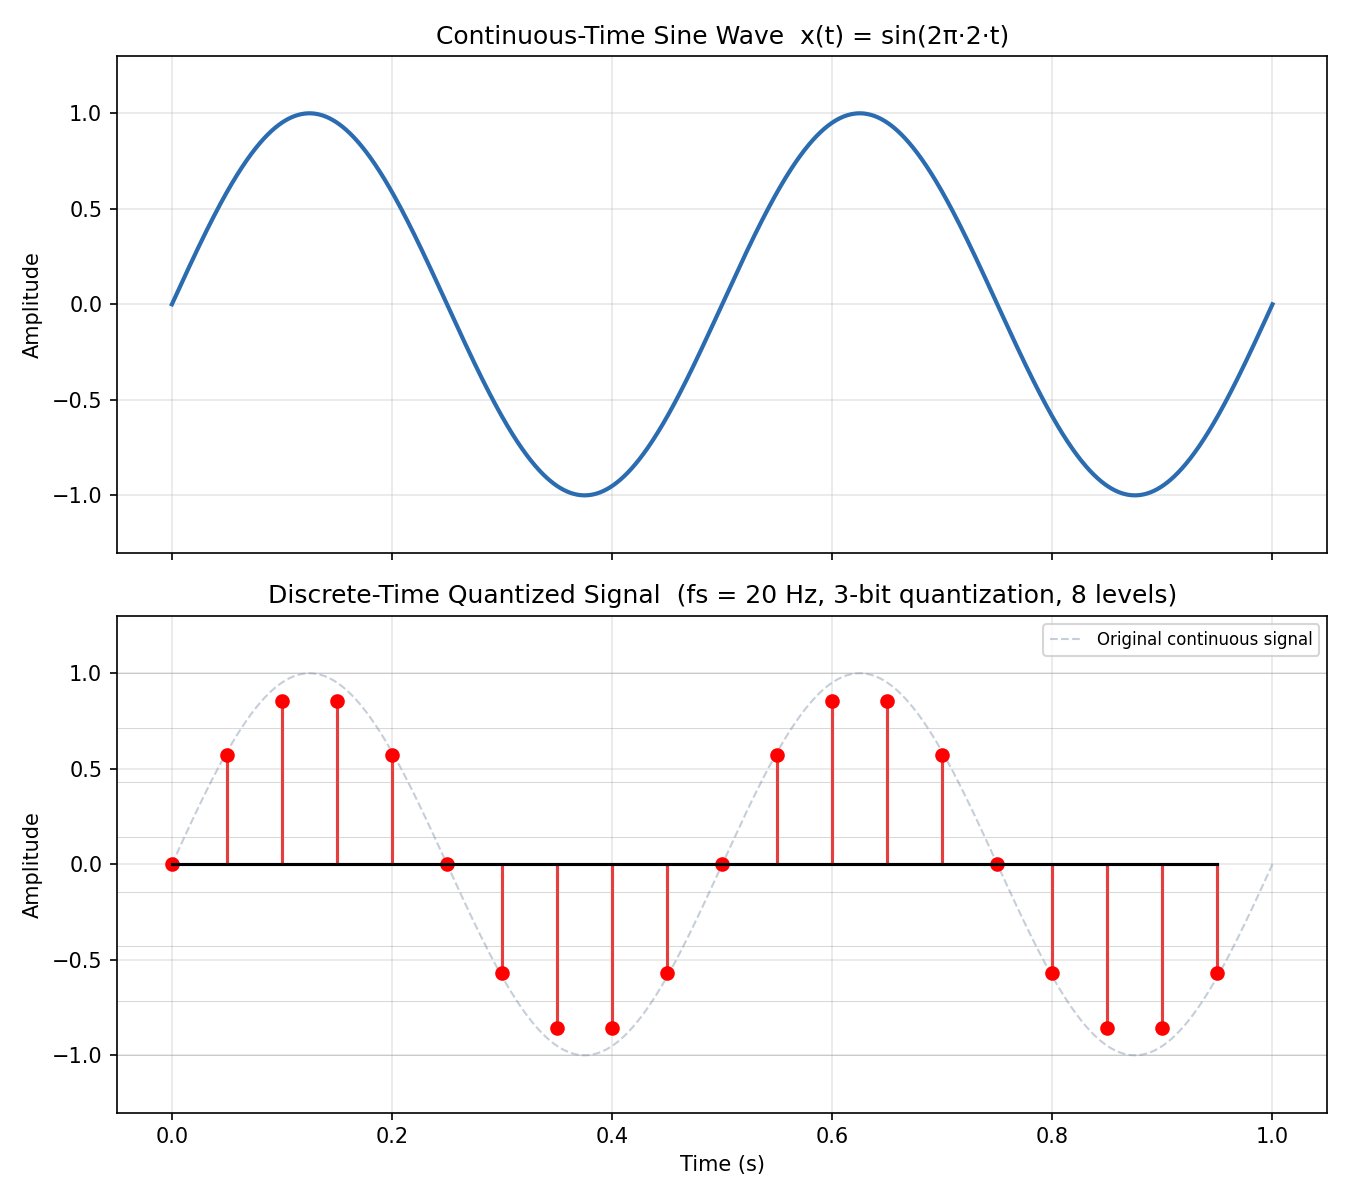
\includegraphics[width=\linewidth]{discussion/audio_basics/figures/sine_wave_quantization.png}
  \caption{Quantization of the continuous time signal to discrete time signals \cite{anthropicclaude}}
  \label{fig:sine_wave_quantization}
\end{figure}

PortAudio is used in the project for audio playback and recording. It utilizes an API that iterates through an array of samples
using a simple callback function that runs periodically until the application stops running. Given the sampling rate, and using the above
example of the sine wave (\Cref{fig:sine_wave_quantization}), the following example (\Cref{prompt:example_float_values}) \cite{anthropicclaude} 
shows a series of samples the callback function would iterate through: 

\begin{verbatim}
0.000000  0.571429  0.857143  0.857143
...
0.571429  0.857143  0.857143  0.571429  0.000000
\end{verbatim}

The program iterates through these samples at a time interval of $T = 1/f_s$. Using such samples provides the ability
to shape and mold wave signal in all forms. Which is why it makes it much easier to model audio signals using mathematical
equations derived from textbooks.

% Subsections
\subsubsection{Choice of Sampling Rate}

According to Nyquist's theorem, the maximum frequency ($f_{\text{max}}$) that the DSP system can analyze needs to be 
half the sampling rate. And it is described by the following equation \cite{siemens_dsp_sampling}:

\begin{equation}
    f_s \geq 2 f_{\text{max}}
\end{equation}

The upper limit of the audible range of a human ear is at \SI{20}{\kilo \hertz}. So the sampling rate
needs to be at least \SI{40}{\kilo \hertz} to prevent aliasing, or any unwanted distortion. Therefore,
\SI{44.1}{\kilo \hertz} is wide adapted as a standard for music production and writing them in 
CDs \cite{lisacademy2026digitalaudio}.
\subsubsection{Using Samples for Scheduling}

It is known from equation \eqref{eq:time_duration} that the number of samples 
define duration. Assuming that the sampling rate remains fixed, it provides a useful 
metric for timestamping and scheduling MIDI events, whenever a melody is written. 
For example, given the sample rate ($f_s$), and the tempo in BPM, the time duration 
of one beat in samples is estimated using the following equation:

\begin{equation}
    t = \left\lfloor f_s \times  \frac{60}{\text{BPM}} \right\rfloor
\end{equation}

For example, if a music is played at 80 BPM, and the sample rate is \SI{44.1}{\kilo \hertz},

$$
    t = \left\lfloor 44100 \times \frac{60}{80} \right\rfloor = 33075
$$

This means that 33,075 samples are required to make one beat. However, the length of one 
music note is not limited to one beat.

Using the same tempo and sampling rate, when a note is scheduled at the 3rd beat, it needs to wait until
the first $33075 \times 2 = 66150$ samples are processed.

This makes it very useful during mixing all the tracks using samples, just to keep the timings
consistent without any interruption. It was initially thought of using \texttt{sleep\_for()} from
the C++ \texttt{std::chrono} library, which pauses an execution for a certain amount of time.
However, this introduces complexities which might require creating enormous amount of threads. Sometimes, they could halt
any high-priority callbacks which may cause bugs. But most importantly, sometimes \texttt{sleep\_for()}
can block for longer than the specified duration due to OS-related scheduling and resource contention 
\cite{cppreference_sleep_for}, which is not real-time friendly by any means. 

To further support this statement, audio hardware already provides the most accurate clock
in the system (\Cref{prompt:chronovssample}) \cite{openai_chatgpt}. Therefore, the audio callback 
timing using the number of samples provides an accurate scheduling of each MIDI events in the 
audio engine.
\subsubsection{Latency and Buffer}

To project analog vibrations to the speakers,  the audio hardware needs to convert this digital signal to
continuous analog voltage using Digital-to-Analog Conversion (DAC). And vice-versa for the microphones using
Analog-to-Digital (ADC) converter. \Cref{fig:latency_signal_flow} presents a simplified signal flow diagram illustrating 
the sources of latency in a digital audio system consisting of ADC and DAC conversion down to buffering and 
processing \cite{burg2014latency}.

\begin{figure}[ht]
  \centering
  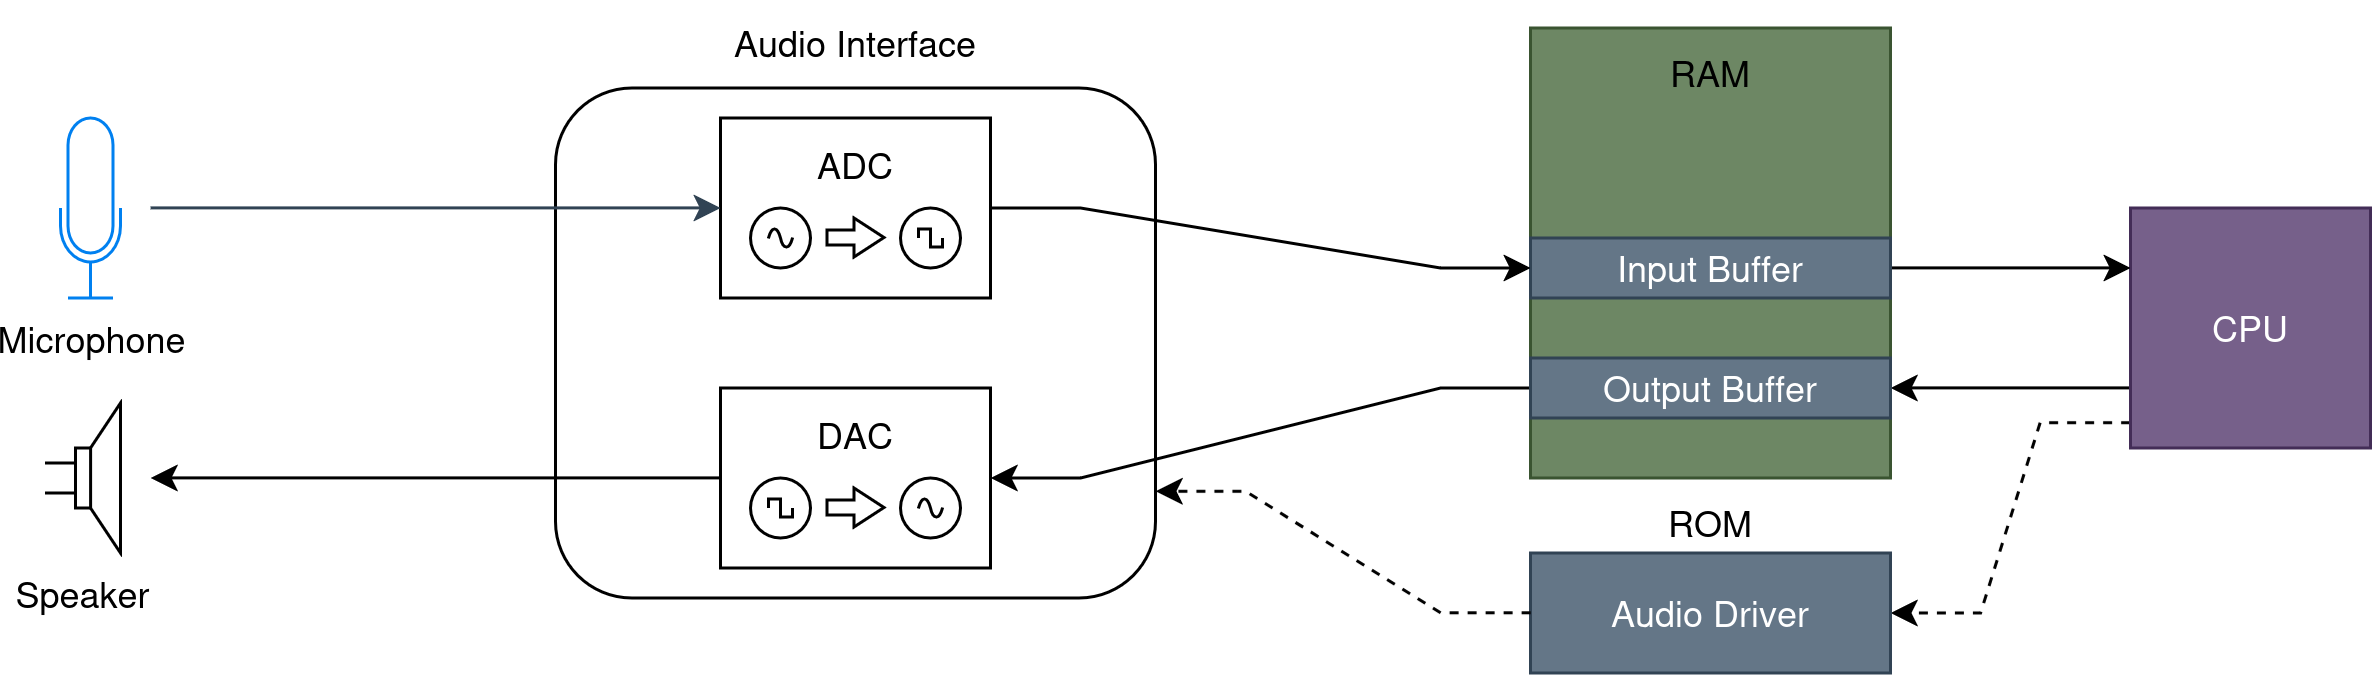
\includegraphics[width=\linewidth]{discussion/audio_basics/figures/SignalFlowDiagramDAC.drawio.png}
  \caption{Signal flow during the latency period \cite{burg2014latency}}
  \label{fig:latency_signal_flow}
\end{figure}

This introduces some latency at regular intervals which causes this delay. However, there are other contributing factors which leads
to such delays (\Cref{prompt:latency_factors}) \cite{openai_chatgpt}:

\begin{itemize}
    \item \textbf{Driver / OS scheduling}: Transfer of data between the audio driver and the application
    \item \textbf{DAW Software Processing}: Time taken by the callback or audio engine to synthesize audio and apply DSP 
    (EQ, convolution, compressors, etc.). It depends on the complexity, which is discussed in the later subsections.
    \item \textbf{I/O Buffer Size}: The larger the number of samples queued, the more time it takes to process those signals 
\end{itemize}

The buffer size is one of the largest contributors to latency, i.e. the time taken to process all the samples after being 
queued to a block of memory. Using solely the buffer size, the latency can be modelled using the equation \cite{burg2014latency}:

\begin{equation}\label{eq:buffer_latency}
    t_{\text{buffer}} = \frac{ N_{\text{buffer}} }{f_s}
\end{equation}

Where $N_{\text{buffer}}$ is the buffer size, and $f_s$ is the sampling frequency. For example, for a buffer size of 256 
samples and a sample rate of 48 kHz, the buffer duration would be,

$$
\frac{256}{48000} \approx \SI{5.33}{\milli \second}
$$
\subsubsection{Computational Time Requirements}
\label{sec:comp_req}

To maintain audio quality in real-time, the deadline must meet the processing requirements, the audio engine
needs to finish processing to synthesize audio and apply DSP within the buffer period \cite{zhao2024multithreaded}, 
until the next chunk of samples are processed. Derived from Rate Monotonic Scheduling theory (\Cref{prompt:execution_time}) 
\cite{openai_chatgpt}, the ratio ($U$) between the callback execution time, $C$ and the buffer duration ($t_{\text{buffer}}$)
determines the the real-time processor utilization, representing the portion of the available deadline 
consumed by the audio engine. This is described by the following equation below \cite{liu1973scheduling}:

\begin{equation}\label{eq:execution_time}
    U = \frac{C}{t_{\text{buffer}}}
\end{equation}

The processing time satisfies the deadline requirements, if and only if $C < t_{\text{buffer}}$ or $U < 1$.
Otherwise, it will lead to glitches (observed through clicks and pops) and some unwanted artifacts.

Design a real-time friendly audio engine with DSP, it must maintain real-time constraints, which includes
avoiding any function calls that takes a longer period of time to execute. These might include the following \cite{portaudio}:
\begin{itemize}
    \item Memory allocation/deallocation
    \item I/O (e.g. \texttt{printf()}, \texttt{std::cin}, etc.)
    \item Context switching (e.g. \texttt{exec()}, or \texttt{yield()})
    \item Any mutex operations
    \item Any tasks related to the operating system
    \item Functions with too much time complexity
\end{itemize}

\Cref{app:exec_time} shows the code listings which measures the callback execution times using \texttt{std::chrono::high\_resolution\_clock::now()}. 
It takes multiple readings for as long as the audio engine runs, which are useful for statistical analysis. This includes the mean, 
maximum (worst-case execution time), and the standard deviation (determines consistency). If the mean or maximum callback time is greater 
than the buffer duration, then there are glitches present during the stream, so it either is a performance issue or a bug needs to 
be fixed.

A numerically different approach for calculating the standard deviation is conducted using the accumulation 
of the sum of callback times, and the squared callback times on to a single variable,
instead of an array or \texttt{std::vector}. The following equation determines this standard deviation \Cref{prompt:stddev}
\cite{haas2022sumofsquares,openai_chatgpt}:

\begin{equation}\label{eq:stddev}
    \sigma = \sqrt{ \frac{\sum x^2 - \frac{\left(\sum x\right)^2}{n} }{n - 1} }
\end{equation}

A larger standard deviation indicates larger variations in time, which means more jitter.

\Cref{app:exec_time}, Listing \ref{lst:raii-timer} shows another way of measuring time, which utilizes the RAII (Resource Acquisition Is Initialization)
technique by taking the start and end times at the constructor and destructor, and calculating the elasped time
after the object is destroyed \cite{nagi2026timingcpp}.


% Using thread sleeping/waiting mechanisms based on durations (which are often paired with std::chrono) does not provide hard timing guarantees because the OS scheduler can delay execution.

% We use samples for real-time scheduling because audio hardware already provides the most accurate clock in the system. std::chrono measures wall-clock time; samples represent the exact timeline of the audio stream.

% samples are not inherently a clock. They become a clock because the sampling rate is fixed. A sequence of samples without knowing fs
% has no absolute time information.

% The sample index is used as a timing metric because the sampling clock establishes a fixed temporal relationship between consecutive samples. Therefore, elapsed audio time can be represented as a number of samples, with conversion determined by the sampling rate.



% References:
% sleep_for cannot be used: https://en.cppreference.com/cpp/thread/sleep_for?utm_source=chatgpt.com

% TODO: Add this prompt: ``Why do we use samples for real-time scheduling instead of std::chrono?''
